\chapter{Data Distribution Service}
\section{Overview}
The concept of distributed applications is to enable seamless communication between systems. There are a number of different ways to achieve this and the one we are focusing on is Data distribution service for real-time systems (DDS).
It is a standard developed by Object Management Group (OMG) that enables communication between computers, that is decoupled in space, time and flow. This means that the computers don't have to know each other and they don't have to be ready to receive when a message is sent. It uses a publish/subscribe pattern to send and receive messages that can be customised by a list of quality of service parameters.

\section{Middleware}
To achieve this seamless communication some layer of software is needed to handle the network communication and distribution of data. This layer of software is called middleware.

Middleware can be defined by this quote:

"A layer of software residing on every machine, sitting between the
underlying operating system and the distributed applications,
whose purpose is to mask the heterogeneity of the cooperating
platforms and provide a simple, consistent and integrated
distributed programming environment."\footnote{Coulouris, G., J. Dollimore, T. Kindberg, and G. Blair (2001). Distributed systems: Concepts and design. Pearson.}

\subsection{What and why?}


\begin{center}
	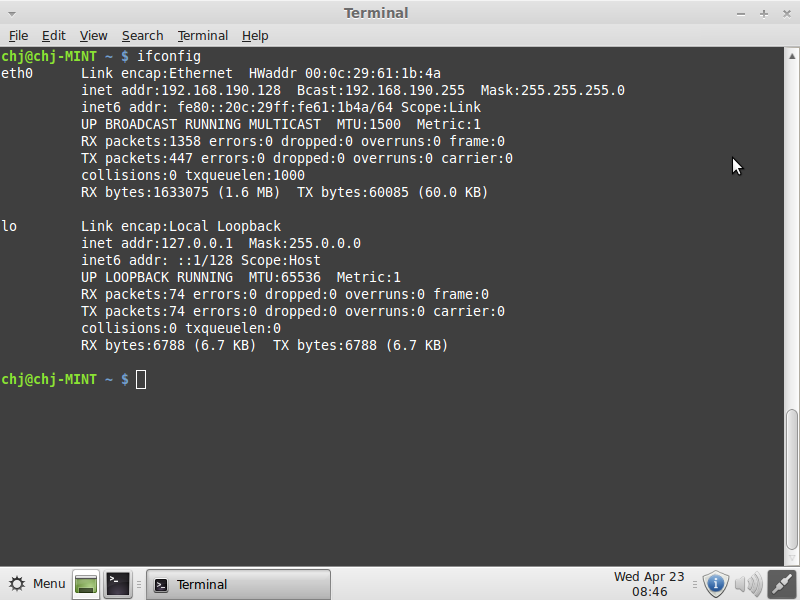
\includegraphics[width=\textwidth]{ifconfig.png}
	\captionof{figure}{Eksempel på billede}
\end{center}

\subsection{Decoupling}



\subsection{Publish/Subscribe pattern}


\subsection{Real-time systems}

\section{Quality Of Service}
For setting up the connections between entities, Publishers, Middleware and Subscribers must agree on certain terms. Quality of Service (QoS) lets the middleware know how to treat connections between publishers and subscribers as well as how to treat messages.

The QoS lets us setup \textit{terms} of the communication. This can be used, for instance, to set up the \textit{lifetime} of a message. This way, we could make sure a message will stop being interesting to subscribers after a while. 

Another example is setting the \textit{deadline} parameter on a subscribers QoS. This tells publishers, that the subscriber expects data within the specified timeframe. This way, if the middleware detects a QoS of the publisher, which will transfer data at a slower rate than what the subscriber requests, the middleware will \textbf{not} connect these two.

The QoS can be set programmatically through properties and structs in the respective classes or through XML configuration files. 

\section{Connext RTI}

\subsection{Configuration on linux}